\documentclass[tikz, border=10pt]{standalone}
\usetikzlibrary{shapes.geometric, arrows.meta, positioning, calc}

% ==================== WIKIMEDIA CODEX COLOUR PALETTE ====================
% Codex Progressive Blue family (Primary System)
\definecolor{codex-blue}{HTML}{3366CC}         % color-progressive (blue700)
\definecolor{codex-blue-light}{HTML}{E8EEFF}   % background-color-progressive-subtle (blue50)
\definecolor{codex-blue-mid}{HTML}{3056A9}     % color-progressive--hover (blue800)
\definecolor{codex-blue-dark}{HTML}{233566}    % color-progressive--active (blue900)

% Codex Success Green family (Secondary Accent / Search & Results)
\definecolor{codex-green}{HTML}{177860}        % color-success (green700)
\definecolor{codex-green-light}{HTML}{DFF2EB}  % background-color-success-subtle (green50)
\definecolor{codex-green-mid}{HTML}{099979}    % color-icon-success (green500)
\definecolor{codex-green-dark}{HTML}{0B5242}   % Dark green for borders and text

% Neutral UI
\definecolor{codex-border}{HTML}{A2A9B1}       % border-color-base (gray400)
\definecolor{codex-neutral-subtle}{HTML}{F8F9FA} % background-color-neutral-subtle (gray50)

% Dark Code block theme (kept dark for high readability of code syntax)
\definecolor{code-bg}{HTML}{1E1E2E}       
\definecolor{code-fg}{HTML}{CDD6F4}       

% VSCode-style syntax colours (for code snippets)
\definecolor{py-keyword}{HTML}{C586C0}
\definecolor{py-variable}{HTML}{9CDCFE}
\definecolor{py-function}{HTML}{DCDCAA}
\definecolor{py-string}{HTML}{CE9178}
\definecolor{py-number}{HTML}{B5CEA8}
\definecolor{py-operator}{HTML}{E0E0E0}

\begin{document}
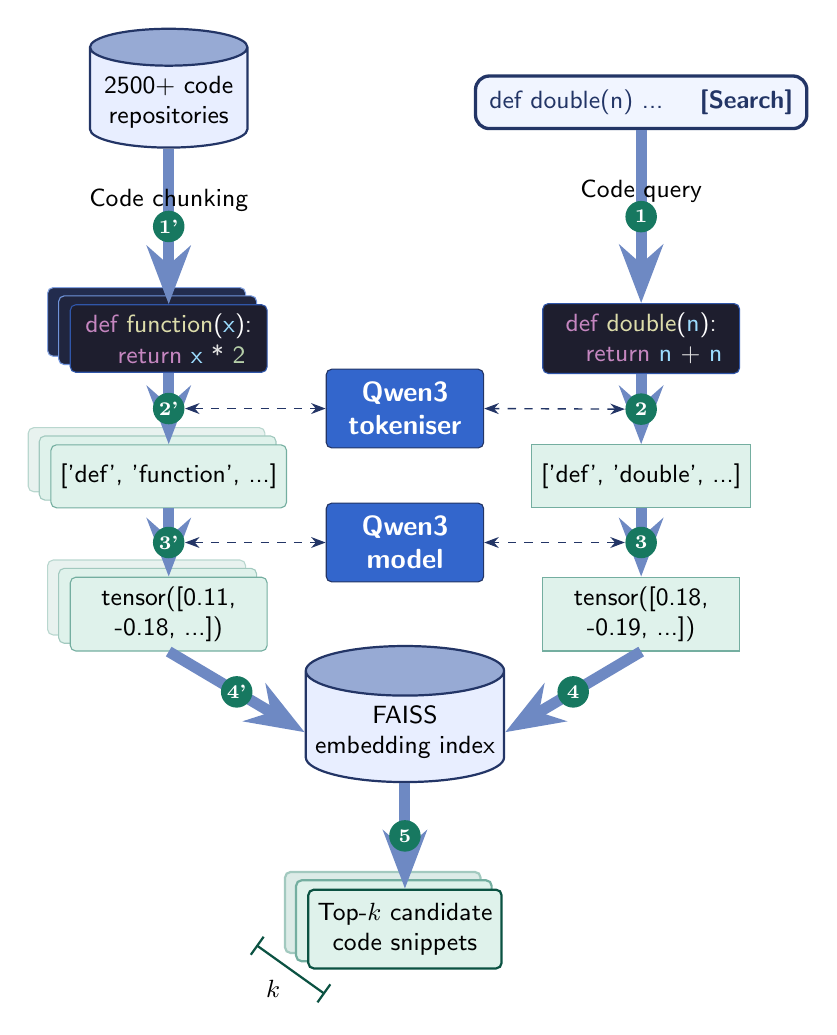
\begin{tikzpicture}[
    font=\sffamily\small,
    >=Stealth,
    % ==================== STYLE DEFINITIONS ====================
    database/.style={
        cylinder, cylinder uses custom fill,
        cylinder body fill=codex-blue-light, cylinder end fill=codex-blue-mid!50,
        shape border rotate=90, draw=codex-blue-dark, thick,
        aspect=0.25, minimum width=2cm, minimum height=1cm, align=center
    },
    block/.style={
        rectangle, draw=codex-blue-dark, fill=codex-blue,
        text=white, font=\sffamily\bfseries,
        minimum width=2cm, minimum height=1cm, align=center, rounded corners=2pt
    },
    databox/.style={
        rectangle, draw=codex-green!60, fill=codex-green-light,
        minimum width=2.5cm, minimum height=0.8cm, align=center
    },
    databox-stack/.style={
        rectangle,
        draw=codex-green!60,
        fill=codex-green-light,
        font=\sffamily\small,
        text=black,
        align=center,
        minimum width=2.5cm,
        minimum height=0.8cm,
        rounded corners=2pt,
        append after command={
            \pgfextra{
                \draw[draw=codex-green!30, fill=codex-green!10, rounded corners=2pt]
                ([shift={(-8pt,6pt)}]\tikzlastnode.north west) rectangle
                ([shift={(-8pt,6pt)}]\tikzlastnode.south east);
                \draw[draw=codex-green!40, fill=codex-green-light, rounded corners=2pt]
                ([shift={(-4pt,3pt)}]\tikzlastnode.north west) rectangle
                ([shift={(-4pt,3pt)}]\tikzlastnode.south east);
            }
        }
    },
    codebox/.style={
        rectangle,
        draw=codex-blue-mid,
        fill=code-bg,
        text=white,
        font=\sffamily\small,
        minimum width=2.5cm,
        minimum height=0.8cm,
        align=center,
        rounded corners=2pt
    },
    codebox-stack/.style={
        rectangle,
        draw=codex-blue-mid,
        fill=code-bg,
        font=\sffamily\small,
        text=white,
        align=center,
        minimum width=2.5cm,
        minimum height=0.8cm,
        rounded corners=2pt,
        append after command={
            \pgfextra{
                \draw[draw=codex-blue!60, fill=code-bg!80!codex-blue, rounded corners=2pt]
                ([shift={(-8pt,6pt)}]\tikzlastnode.north west) rectangle
                ([shift={(-8pt,6pt)}]\tikzlastnode.south east);
                \draw[draw=codex-blue!70, fill=code-bg!90!codex-blue, rounded corners=2pt]
                ([shift={(-4pt,3pt)}]\tikzlastnode.north west) rectangle
                ([shift={(-4pt,3pt)}]\tikzlastnode.south east);
            }
        }
    },
    % Recall results (bi-encoder output) — green stacked
    results-stack/.style={
        rectangle,
        draw=codex-green-dark,
        fill=codex-green-light,
        thick,
        minimum width=2cm,
        minimum height=1cm,
        align=center,
        rounded corners=2pt,
        append after command={
            \pgfextra{
                \draw[draw=codex-green!40, fill=codex-green!15, thick, rounded corners=2pt]
                ([shift={(-8pt,6pt)}]\tikzlastnode.north west) rectangle
                ([shift={(-8pt,6pt)}]\tikzlastnode.south east);
                \draw[draw=codex-green!60, fill=codex-green-light, thick, rounded corners=2pt]
                ([shift={(-4pt,3pt)}]\tikzlastnode.north west) rectangle
                ([shift={(-4pt,3pt)}]\tikzlastnode.south east);
                \draw[{Bar[width=8pt]}-{Bar[width=8pt]}, codex-green-dark, thick, shorten <=2pt, shorten >=2pt]
                ([shift={(-20pt,10pt)}]\tikzlastnode.south west) --
                ([shift={(8pt,-10pt)}]\tikzlastnode.south west)
                node[midway, below left, black] {$k$};
            }
        }
    },
    arrow_label/.style={
        circle, fill=codex-green, text=white, inner sep=1pt, font=\scriptsize\bfseries, minimum size=4mm
    },
    main_arrow/.style={
        ->, line width=4pt, codex-blue-mid!70
    },
]

% ==================== LEFT SIDE: INDEXING PIPELINE ====================
\node[database] (cms) at (-3, +4) {2500+ code\\repositories};

\node[codebox-stack] (text_in) at (-3, 1) {%
    \textcolor{py-keyword}{def} \textcolor{py-function}{function}(\textcolor{py-variable}{x})\textcolor{py-operator}{:}\\
    \quad \textcolor{py-keyword}{return} \textcolor{py-variable}{x} \textcolor{py-operator}{*} \textcolor{py-number}{2}
};
\node[databox-stack] (tokens_in) at (-3, -0.75) {['def', 'function', ...]};
\node[databox-stack] (tensor_in) at (-3, -2.5) {tensor([0.11,\\-0.18, ...])};

\draw[main_arrow] (cms.south) -- (text_in.north) node[midway, above, black] {Code chunking};
\node[arrow_label] at ($(cms.south)!0.5!(text_in.north)$) {1'};

\draw[main_arrow] (text_in.south) -- (tokens_in.north);
\node[arrow_label] (label2) at ($(text_in.south)!0.5!(tokens_in.north)$) {2'};

\draw[main_arrow] (tokens_in.south) -- (tensor_in.north);
\node[arrow_label] (label3) at ($(tokens_in.south)!0.5!(tensor_in.north)$) {3'};

% ==================== RIGHT SIDE: QUERY PIPELINE ====================
\node[draw, codex-blue-dark, line width=1.2pt, rounded corners=5pt, inner sep=5pt, fill=codex-blue-light!60]
    (search_bar) at (3, 5 |- cms.center) {def double(n) ... \quad \textbf{[Search]}};

\node[codebox] (query_in) at (3, 1 |- text_in.center) {%
    \textcolor{py-keyword}{def} \textcolor{py-function}{double}(\textcolor{py-variable}{n})\textcolor{py-operator}{:}\\
    \quad \textcolor{py-keyword}{return} \textcolor{py-variable}{n} \textcolor{py-operator}{+} \textcolor{py-variable}{n}
};
\node[databox] (q_tokens) at (3, -1.2 |- tokens_in.center) {['def', 'double', ...]};
\node[databox] (q_tensor) at (3, -3.5 |- tensor_in.center) {tensor([0.18,\\-0.19, ...])};

\draw[main_arrow] (search_bar.south) -- (query_in.north) node[midway, above, black] {Code query};
\node[arrow_label] at ($(search_bar.south)!0.5!(query_in.north)$) {1};

\draw[main_arrow] (query_in.south) -- (q_tokens.north);
\node[arrow_label] (label2r) at ($(query_in.south)!0.5!(q_tokens.north)$) {2};

\draw[main_arrow] (q_tokens.south) -- (q_tensor.north);
\node[arrow_label] (label3r) at ($(q_tokens.south)!0.5!(q_tensor.north)$) {3};

% ==================== CENTRAL PROCESSING COMPONENTS ====================
\node[block] (tokeniser) at (0,0 |- label2.center) {Qwen3\\tokeniser};
\node[block] (encoder)   at (0,0 |- label3.center) {Qwen3\\model};

\draw[<->, dashed, codex-blue-dark, line width=0.5pt] (label2.east)  -- (tokeniser.west);
\draw[<->, dashed, codex-blue-dark, line width=0.5pt] (label3.east)  -- (encoder.west);
\draw[<->, dashed, codex-blue-dark, line width=0.5pt] (label2r.west) -- (tokeniser.east);
\draw[<->, dashed, codex-blue-dark, line width=0.5pt] (label3r.west) -- (encoder.east);

% ==================== FAISS INDEX AND RECALL ====================
\node[database, minimum width=2.5cm] (index) at (0, -4) {FAISS\\embedding index};

\draw[main_arrow] (tensor_in.south) -- (index.west);
\node[arrow_label] at ($(tensor_in.south)!0.5!(index.west)$) {4'};

\draw[main_arrow] (q_tensor.south) -- (index.east);
\node[arrow_label] at ($(q_tensor.south)!0.5!(index.east)$) {4};

% Recall results (top-k candidates from bi-encoder)
\node[results-stack] (results) at (0, -6.5) {Top-$k$ candidate\\code snippets};
\draw[main_arrow] (index.south) -- (results.north);
\node[arrow_label] at ($(index.south)!0.5!(results.north)$) {5};

\end{tikzpicture}
\end{document}
